\documentclass{article}
\usepackage{graphicx} % Required for inserting images
\usepackage{float}
\usepackage{hyperref}
\usepackage[a4paper, total={6in, 9in}]{geometry}

\title{CSE556: Natural Language Processing \\ Assignment-1}
\author{Himanshu Raj (2022216) \textbar{} Ishita (2022224) \textbar{} Ritika Thakur (2022408) }
\date{February 2, 2025}

\begin{document}
\maketitle

\section{Task 1}
\subsection{Data Pre-processing}
Our corpus \texttt{corpus.txt} had over \texttt{45k} words which included all lower-case words with no number and punctuations. The corpus also included words like \texttt{http}, \texttt{src}, \texttt{img}, \texttt{href}, \texttt{www} which did not add anything to the contextual meaning of the words.
The following pre-processing steps were applied:
\begin{itemize}
\item \textbf{Removing irrelevant words and trailing content}: Words such as \texttt{img}, \texttt{http}, \texttt{href}, and \texttt{src} along with everything after them were removed to eliminate unnecessary HTML-like tags and URLs. These words along with the trailing content were found to be irrelevant in the corpus and did not add to the context of the sentences.
\item \textbf{Whitespace normalization}: Extra spaces were removed.
\end{itemize}

\begin{figure}[H]
    \centering
    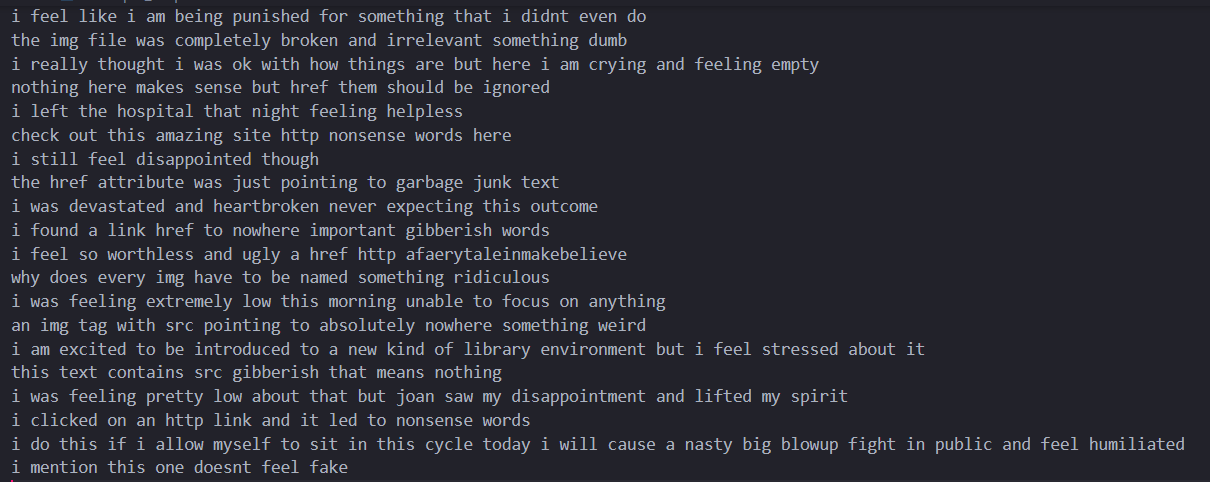
\includegraphics[width=0.75\linewidth]{image1.png}
    \caption{Example corpus before pre-processing}
    \label{fig:enter-task1}
\end{figure}
\begin{figure}[H]
    \centering
    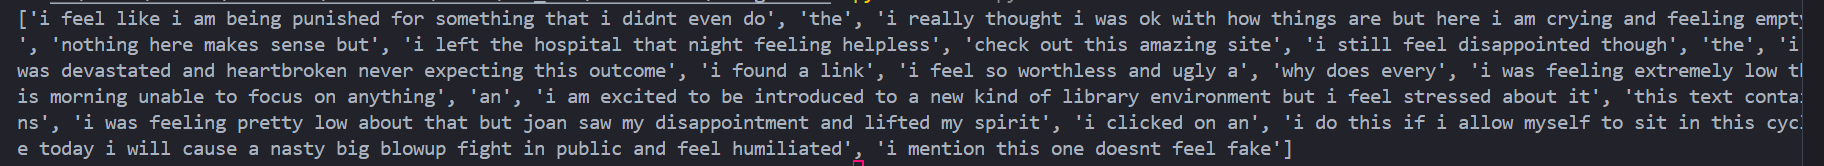
\includegraphics[width=0.75\linewidth]{image2.png}
    \caption{Example corpus after pre-processing}
    \label{fig:enter-task1}
\end{figure}

\subsection{Vocabulary Generation}
The vocabulary generation is based on the WordPiece subword tokenization approach (similar to BPE Algorithm).
\begin{enumerate}
    \item \textbf{Splitting words into characters}: Each word is initially split into individual characters, with non-initial characters prefixed by \texttt{\#\#}.
    \item \textbf{Pair frequency calculation}: The frequency of adjacent character pairs is counted across the corpus.
    \item \textbf{Pair scoring}: A score is calculated for each character pair based on its frequency relative to individual unit frequencies:\\ \texttt{freq\{pair\}} / \texttt{(freq\{word1\} * freq\{word2\})}
    \item \textbf{Merging pairs iteratively}: The highest-scoring pairs are merged until the vocabulary size reaches the predefined limit.
\end{enumerate}
\texttt{[UNK]} and \texttt{[PAD]} are also added to the vocabulary.

\begin{figure}[H]
    \centering
    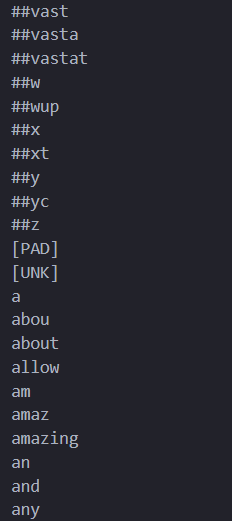
\includegraphics[width=0.35\linewidth]{image4.png}
    \caption{Snippet from vocabulary generated from example corpus with \texttt{size=500}}
    \label{fig:enter-task1}
\end{figure}
% \begin{figure}[H]
%     \centering
%     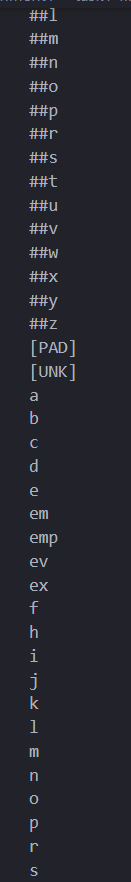
\includegraphics[width=0.25\linewidth]{image3.png}
%     \caption{Snippet from vocabulary generated from example corpus with \texttt{size=50}}
%     \label{fig:enter-label}
% \end{figure}

\subsection{Tokenization}
The tokenization process converts input text into subword units based on the generated vocabulary. After splitting words in the text into characters, as done during vocabulary generation, characters are merged based on the longest match in the vocabulary. If a word cannot be matched, it is replaced with \texttt{[UNK]}.

\begin{figure}[H]
    \centering
    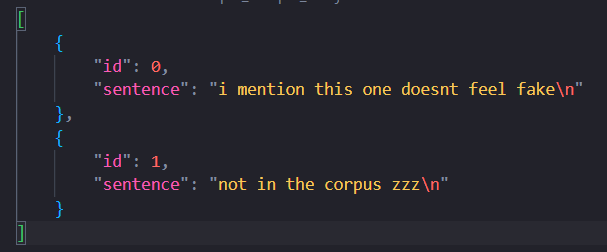
\includegraphics[width=0.5\linewidth]{image5.png}
    \caption{Test json file}
    \label{fig:enter-task1}
\end{figure}
\begin{figure}[H]
    \centering
    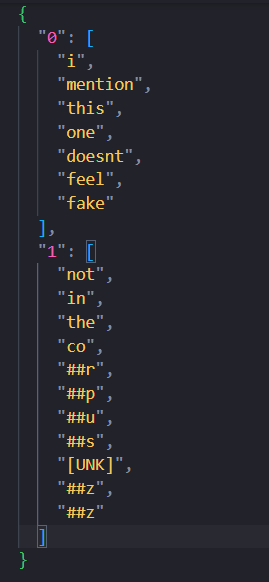
\includegraphics[width=0.25\linewidth]{image6.png}
    \caption{Tokenized json file}
    \label{fig:enter-task1}
\end{figure}

\section{Task 2}

\subsection{Introduction}

We build a Word2Vec model using the Continuous Bag of Words (CBOW) approach. The goal is to preprocess the input text corpus, generate CBOW pairs, and use them to train the Word2Vec model. Also, we find similar and dissimilar word triplets using cosine similarity.

\subsection{Dataset Preparation - Word2VecDataset Class}
The \textbf{Word2VecDataset class} preprocesses the input text corpus  for training the Word2Vec model using the \textbf{Continuous Bag of Words (CBOW)} approach.

\begin{enumerate}
\item \textbf{Initialization} : It initializes the window size for context words, vocabulary, and mappings between words and indices (word2idx and idx2word). It also initializes CBOW training pairs.

\item \textbf{Pre-processes Data} : 
    \begin{enumerate}
        \item Uses the WordPieceTokenizer from Task 1 to generate the vocabulary from the input text.
        \item Tokenizes the input text corpus using the WordPieceTokenizer from Task 1.
        \item Generates mapping from each word to a unique index and vice versa
        \item Generates CBOW training pairs based on the tokenized corpus.
    \end{enumerate}
    
\end{enumerate}

\begin{figure}[H]
    \centering
    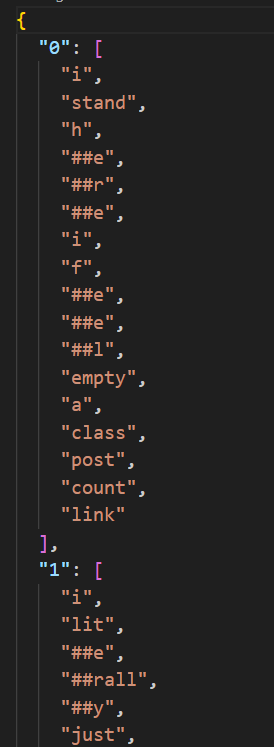
\includegraphics[width=0.18\linewidth]{image7.png}
    \caption{Tokenized Corpus}
    \label{fig:enter-task1}
\end{figure}
\begin{figure}[H]
    \centering
    % \hspace*{-0.1\linewidth} % Adjust this value to move the image left
    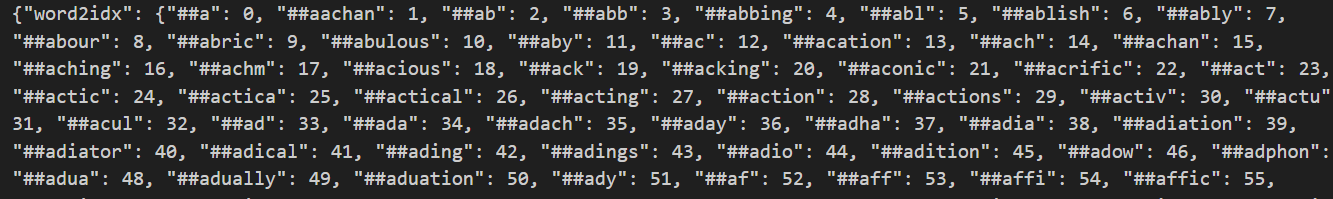
\includegraphics[width=1\linewidth]{image8.png} % Increase the width as needed
    \caption{Word to Index Mapping}
    \label{fig:enter-task1}
\end{figure}

\begin{figure}[H]
    \centering
    % \hspace*{-0.2\linewidth} % Adjust this value to move the image left
    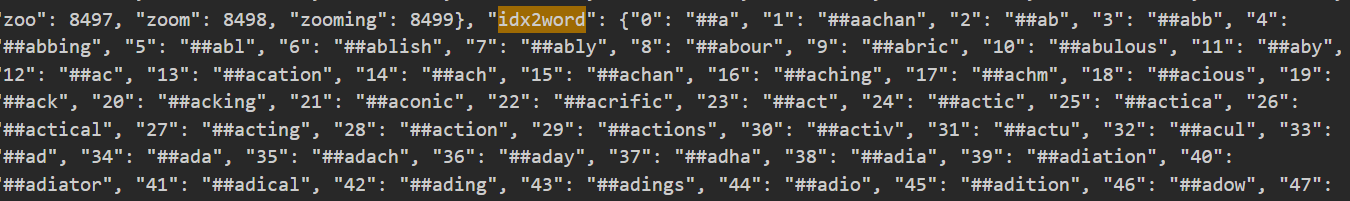
\includegraphics[width=1\linewidth]{image9.png} % Increase the width as needed
    \caption{Index to Word Mapping}
    \label{fig:enter-task1}
\end{figure}

\subsection{Model Architecture - Word2VecModel Class}
\begin{enumerate}
\item \textbf{Initialization} : Initializes the vocabulary size, embedding dimension for each word and weights using a uniform distribution. Bias terms are set to zero.
\item \textbf{Architecture Details}

\begin{itemize}
\item \textbf{Embedding Layer}: Maps words to their corresponding vector representations.
\item \textbf{Linear Layer}: Predicts the target word given the context of word embeddings.
\item \textbf{Log Softmax Activation}: Outputs probability distribution over the entire vocabulary.
\end{itemize}

\item \textbf{Forward Function} : The forward pass gets the embeddings for the context words, averages them, and sends the result to the output layer. The softmax function is then applied to give a probability distribution over all the words in the vocabulary.
\item \textbf{Calculates Cosine Similarity} : Calculates cosine similarity between two vectors and also identifies the most and least similar vector to a given vector.

\end{enumerate}


\subsection{Training}

\begin{enumerate}

\item \textbf{Initialization} : Initializes Adam optimizer, NLLLoss() for calculating loss and moves the model to the appropriate device (CPU/GPU). At the same time it also initializes history to keep track of loss and accuracy.

\item \textbf{Training} : The function trains the Word2Vec CBOW model. In every iteration, it decreases the learning rate and processes batches of context-target pairs. For each batch, the model performs a forward pass, computes the loss, and applies backpropagation to update the weights. Training progress, including batch loss and accuracy, is displayed using the progress bar.
\item \textbf{Model Validation} : After each epoch it computes validation loss, validation accuracy and average cosine similarity for the batch and updates the history.

\item \textbf{Updates Final Checkpoint and Saves the Final Model}
\end{enumerate}

\subsection{Finding Triplets}
The \textbf{find\_triplets} function creates triplets consisting of two similar words and one dissimilar word based on cosine similarity. It randomly selects a word, retrieves the two most similar words, and identifies the least similar word using the Word2Vec model.

\paragraph{Triplet 1:}
\begin{itemize}
    \item \textbf{High positive similarity:} "\#run" has a similarity of \textbf{0.8747} with "haul" and \textbf{0.8696} with "\#ashion"  ighlighting their frequent occurrence in similar contexts.
    \item \textbf{Negative similarity:} "\#run" and "uhur" have a similarity of \textbf{-0.9269}, suggesting they occur in opposite contexts or are rarely used together.
\end{itemize}

\paragraph{Triplet 2:}
\begin{itemize}
    \item \textbf{Very high positive similarity:} "\#logic" has a similarity of \textbf{0.9312} with "\#\#rful" and \textbf{0.9026} with "entry," highlighting their frequent occurrence in similar contexts.
    \item \textbf{Negative similarity:} "\#logic" and "\#aomi" have a similarity of \textbf{-0.8795},suggesting they occur
in opposite contexts or are rarely used together.
\end{itemize}

\begin{figure}[H]
    \centering
    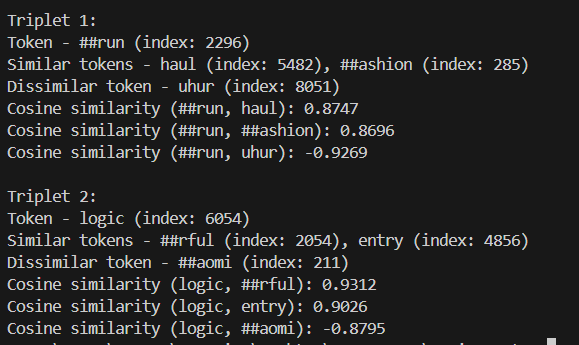
\includegraphics[width=0.65\linewidth]{image12.png}
    \caption{Identifying Triplets}
    \label{fig:enter-task1}
\end{figure}

\subsection{Experimental Results}
After experimenting with the values of hyperparameters, the following hyperparameters gave the best results:

\begin{description}
    \item WINDOW\_SIZE = 4
    \item EMBEDDING\_DIM = 10
    \item BATCH\_SIZE = 256
    \item NUM\_EPOCHS = 15
    \item LEARNING\_RATE = 0.02
    \item TRAIN\_SPLIT = 0.8
    \item VOCAB\_SIZE = 8500
\end{description}
\begin{figure}[H]
    \centering
    % \hspace*{-0.3\linewidth} % Adjust this value to move the image left
    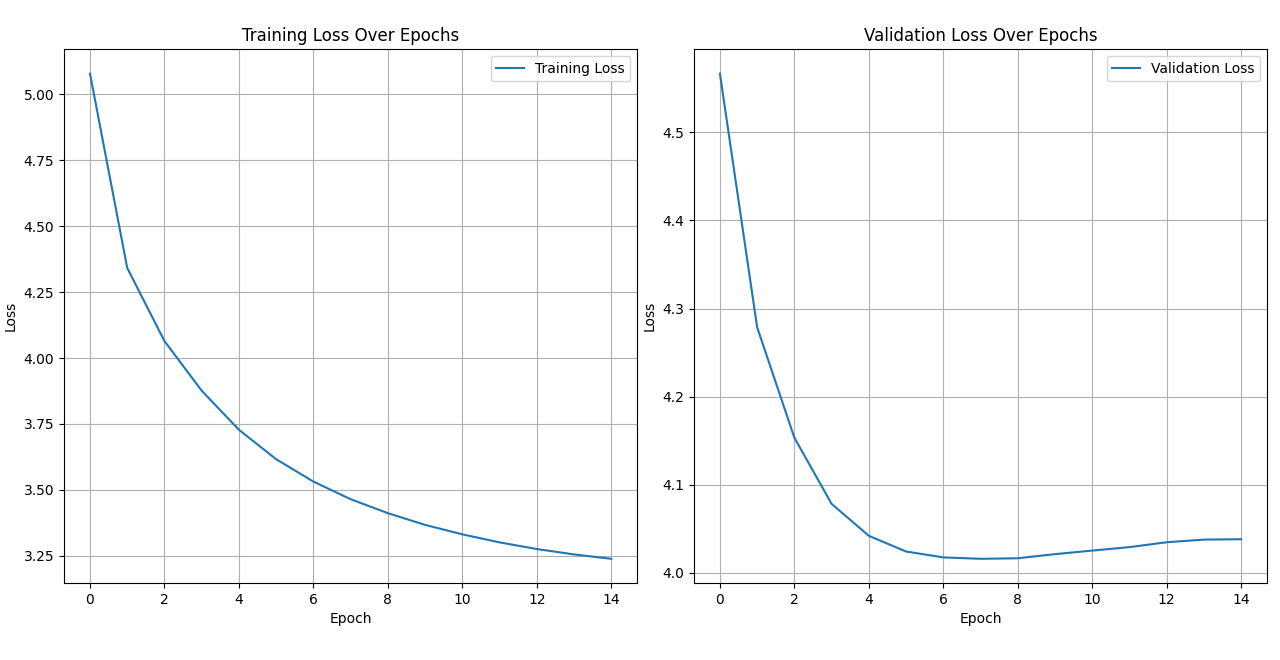
\includegraphics[width=1\linewidth]{image10.png} % Increase the width as needed
    \caption{Training Loss and Validation Loss}
    \label{fig:enter-task1}
\end{figure}
\begin{figure}[H]
    \centering
    % \hspace*{-0.1\linewidth} % Adjust this value to move the image left
    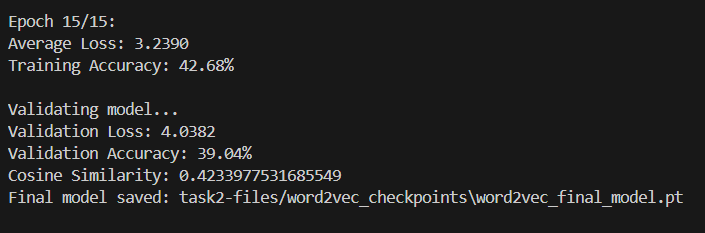
\includegraphics[width=0.75\linewidth]{image11.png} % Increase the width as needed
    \caption{Best Validation Accuracy using the given hyperparameters}
    \label{fig:enter-task1}
\end{figure}

\section{Task 3}

\subsection{Introduction}
For all architectures, input layer contains 40 neurons (context$_$window x embedding$_$dimension = 4x10) and output layer contains 8500 neurons (the vocab size used to train Word2Vec model). All models were trained for 5 epochs with a learning rate of 0.01 with a batch size of 1024 samples over a training set with 60,000+ samples. A common observation over these models was that validation loss increased significantly after 6th epoch, even with smaller learning rates. The training time and compute increased as we go from NeuralLM1 to NeuralLM2 to NeuralLM3.

\subsection{Design Justifications and Performance comparisons}
\textbf{NeuralLM1}: 1 hidden layer with 1024 neurons and tanh activation\\
\\
Justification: This is a basic MLP based Neural Language Model architecture proposed by Bengio in 2003. This serves as a good baseline model to start with when training neural language models.
\\ \\
\textbf{NeuralLM2}: 1 hidden layer with 1024 neurons and ReLU activation and skip connection\\
\\
Justification: The tanh activation outputs cap at a value of 1 which can lead to less/slower updates in learnable parameters. The ReLU activation output is unbounded and hence is used in an attempt to improve accuracy and perplexity. Skip connections help in tackling vanishing gradients, proposed by Bengio in 2003 but they were optional.\\
\\
Improvement: This led to better training and validation accuracy than NeuralLM1. Training perplexity decreased, but validation perplexity increased signifying model is unable to generalize on unseen data.
\\ \\
\textbf{NeuralLM3}: 2 hidden layers with 512 and 2048 neurons and ReLU activation\\
\\
Justification: In previous 2 architectures, validation loss increases after 6th epoch indicating model is unable to generalize on unseen data. Hence, another hidden layer is introduced in an attempt to capture the features in a better way, so that the model can generalise well on unseen data. We are not adding skip connection like NeuralLM2 because we saw an increase in validation perplexity because of which model is unable to generalize well on unseen data.\\
\\
Improvement: This led to better training and validation accuracy than NeuralLM2. The validity perplexity is even less than NeuralLM1, signifying the best performance on unseen data out of all architectures. Training perplexity is a bit more than NeuralLM2, but still less than NeuralLM1.


\subsection{Loss vs Epoch graphs}
\begin{figure}[H]
    \centering
    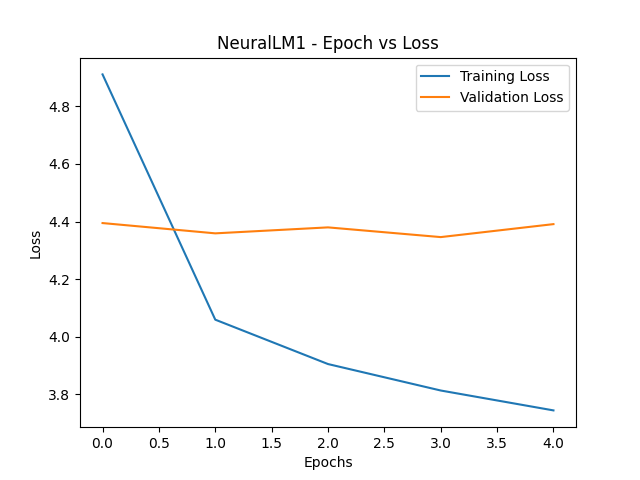
\includegraphics[width=0.5\linewidth]{NeuralLM1Loss.png}
    \caption{Loss vs Epoch curve for NeuralLM1}
\end{figure}

\begin{figure}[H]
    \centering
    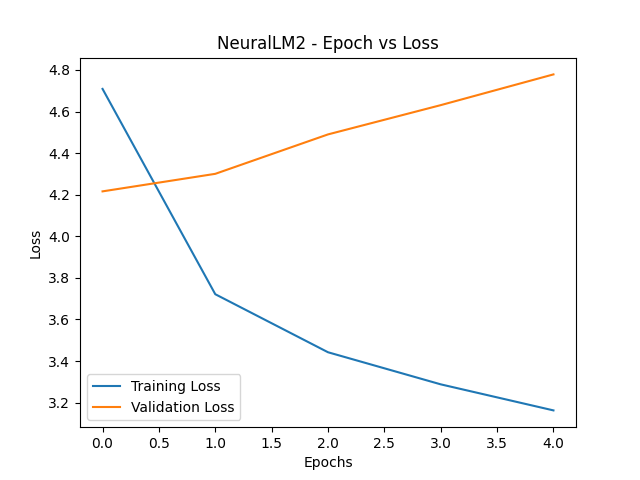
\includegraphics[width=0.5\linewidth]{NeuralLM2Loss.png}
    \caption{Loss vs Epoch curve for NeuralLM2}
\end{figure}

\begin{figure}[H]
    \centering
    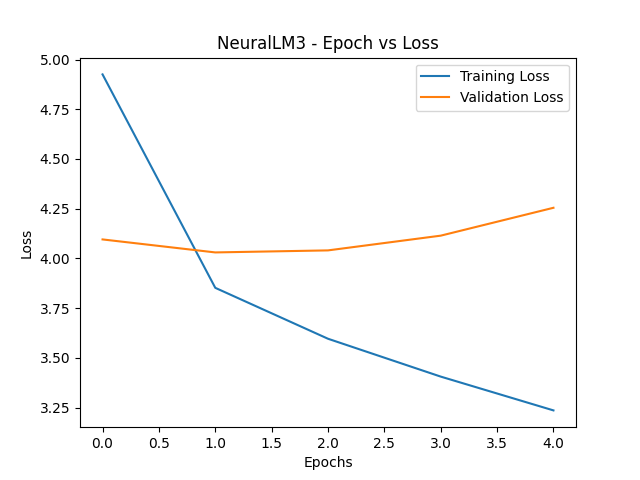
\includegraphics[width=0.5\linewidth]{NeuralLM3Loss.png}
    \caption{Loss vs Epoch curve for NeuralLM3}
\end{figure}


\subsection{Accuracies and Perplexity scores}

\begin{table}[h]
    \centering
    \begin{tabular}{|c|c|c|c|c|}
        \hline
        \multirow{}{}{Model} & \multicolumn{2}{c|}{Accuracy} & \multicolumn{2}{c|}{Perplexity} \\
        \cline{2-5}
        & Training & Validation & Training & Validation \\
        \hline
        NeuralLM1 & 36.01\% & 35.97\% & 42.27 & 80.71 \\
        NeuralLM2 & 39.73\% & 37.81\% & 23.63 & 118.94 \\
        NeuralLM3 & 39.17\% & 39.37\% & 25.43 & 70.43 \\
        \hline
    \end{tabular}
    % \caption{A simple table}
    % \label{tab:example}
\end{table}

\begin{figure}[H]
    \centering
    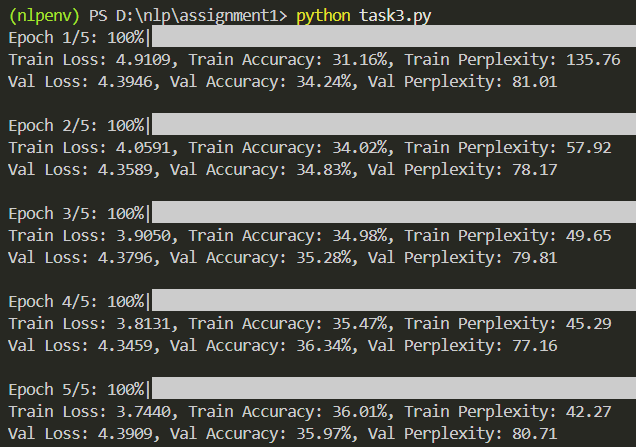
\includegraphics[width=0.5\linewidth]{model1.png}
    \caption{Loss, Accuracy and Perplexity over epochs for NeuralLM1}
\end{figure}

\begin{figure}[H]
    \centering
    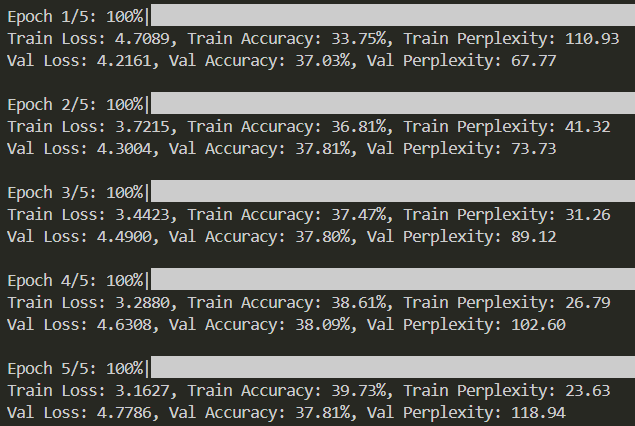
\includegraphics[width=0.5\linewidth]{model2.png}
    \caption{Loss, Accuracy and Perplexity over epochs for NeuralLM2}
\end{figure}

\begin{figure}[H]
    \centering
    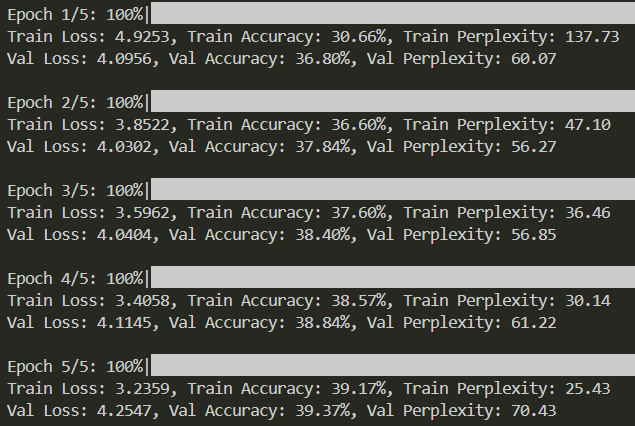
\includegraphics[width=0.5\linewidth]{model3.png}
    \caption{Loss, Accuracy and Perplexity over epochs for NeuralLM3}
\end{figure}


\section{Individual Contribution}
\begin{itemize}
    \item Himanshu Raj: Task 3 implementation and report
    \item Ishita: Task 2 implementation and report
    \item Ritika Thakur: Task 1 implementation and report
\end{itemize}

\section{References}
\begin{itemize}
    \item \href{https://www.youtube.com/watch?v=qpv6ms_t_1A&t=1s}{WordPieceTokenizer Tutorial} 
    \item \href{https://arxiv.org/pdf/1301.3781}{Word2Vec paper}
    \item \href{https://pytorch.org/tutorials/beginner/basics/data_tutorial.html}{Custom dataset Tutorial}
    \item \href{https://github.com/rahisenpai/CSE343-ML/blob/main/asgn4/code_c.ipynb}{PyTorch Implementations}
    \item \href{https://www.researchgate.net/figure/Different-skip-connection-schemes-a-No-skip-connection-b-Distinct-source-skip_fig1_329750500}{Skip-connections}
    \item Lecture Slides - Language Modelling, Word Representation
\end{itemize}

\end{document}